%!TEX root=../../main.tex

\chapter{Inference for numerical data}
\label{inferenceForNumericalData}

\begin{comment}
	
	-- Go back to chapter 4 to emphasize the possible use of software to compute normal probabilities.
	
	-- Do the same thing here when discussing computing t probabilities
	
\end{comment}


Chapter~\ref{foundationsForInference} introduced some of the primary tools of statistical inference -- point and confidence  interval estimates and hypothesis tests.  This chapter examines some scientific settings where these tools are often used, including the analysis of paired observations and comparing two or more independent groups.  The beginning of the chapter returns to the problem of inference for a population mean, adding a new distribution, the $t$-distribution, which can often be used in small samples. 


%__________________
\section{One-sample means with the $t$-distribution}
\label{oneSampleMeansWithTDistribution}

The tools studied in Chapter~\ref{foundationsForInference} all made use of the $t$-statistic from a sample mean:
\[
   t = \frac{\overline{x} - \mu}{s}.
\]
The parameter $\mu$ was a population mean, and $\overline{x}$ and $s$ were the sample mean and standard deviation.  Tests and confidence intervals were restricted to samples of at least 30 independent observations from a population where there was no evidence of strong skewness.  This restriction justified appealing to the Central Limit Theorem to calculate probabilities for the $t$-statistic from the normal probability model. If the data are approximately symmetric and there are no large outliers, the $t$-statistic has what is called a $t$-distribution in sample sizes smaller than 30.  That is where the $t-$statistic gets its name.  Using the normal distribution as the sampling distribution of the $t$-statistic essentially treats $s$ as a good replacement for the unknown population standard deviation, $\sigma$.  The sample standard deviation $s$ is really an estimate of $\sigma$, and has an inherent variability just as $\overline{x}$ does.  The $t$ density function has a shape  similar to the normal density but adjusts for the variability in $s$ by having more probability in the left and right tails -- it has more variability.


\subsection{Introducing the $t$-distribution}
\label{introducingTheTDistribution}

\index{t-distribution|(}
\index{distribution!$t$|(}

A $t$-distribution, shown as a solid line in Figure~\ref{tDistCompareToNormalDist}, has a bell shape. However, its tails are thicker than the normal model's. This means observations are more likely to fall beyond two standard deviations from the mean than under the normal distribution.\footnote{The standard deviation of the $t$-distribution is actually a little more than 1. However, it is useful to always think of the $t$-distribution as having a standard deviation of 1 in all of our applications.} While our estimate of the standard error will be a little less accurate when we are analyzing a small data set, the extra thick tails of the $t$-distribution correct for the variability in $s$. 

\begin{figure}
\centering
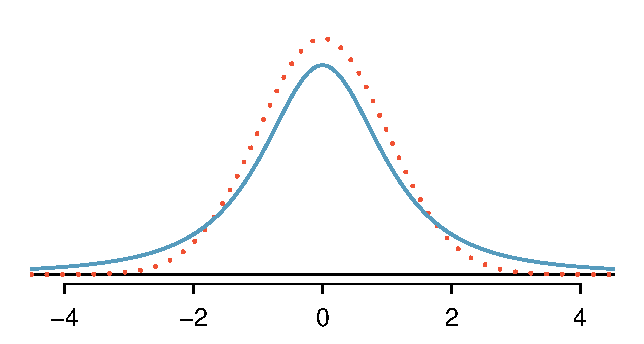
\includegraphics[height=45mm]{ch_inference_for_means_oi_biostat/figures/tDistCompareToNormalDist/tDistCompareToNormalDist}
\caption{Comparison of a $t$-distribution (solid line) and a normal distribution (dotted line).}
\label{tDistCompareToNormalDist}
\end{figure}

The $t$-distribution, always centered at zero, has a single parameter: degrees of freedom.  Several $t$-distributions are shown in Figure~\ref{tDistConvergeToNormalDist}. When there are more degrees of freedom, the $t$-distribution looks very much like the standard normal distribution.

\begin{figure}
\centering
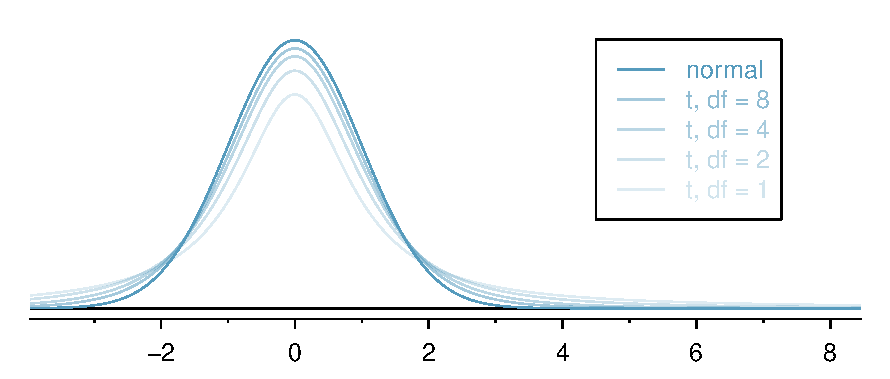
\includegraphics[width=0.8\textwidth]{ch_inference_for_means_oi_biostat/figures/tDistConvergeToNormalDist/tDistConvergeToNormalDist}
\caption{The larger the degrees of freedom, the more closely the $t$-distribution resembles the standard normal model.}
\label{tDistConvergeToNormalDist}
\end{figure}

\begin{termBox}{\tBoxTitle{Degrees of freedom (df)}
The degrees of freedom describe the shape of the $t$-distribution. The larger the degrees of freedom, the more closely the distribution approximates the normal model.}
\end{termBox}

With degrees of freedom about 30 or more, the $t$-distribution is nearly indistinguishable from the normal distribution. The degrees of freedom for the The $t$-statistic in Chapter~\ref{foundationsForInference} has a $t$ distribution with degrees of freedom equal to the sample size - 1, justifying the use of the normal distribution in that chapter.  Section~\ref{tDistSolutionToSEProblem} provides a more complete account of the link between degrees of freedom and sample size.

Probabilities for the $t$-distribution can be calculated using tables of the distribution or using software.  The use of software has become the preferred method because it is more accurate than tables, is not limited to a small range of degrees of freedom and allows complete flexibility in the choice of $t$ values on the horizontal axis.  But each software package uses slightly different commands, so this section illustrates the use of a \term{t-table}, partially shown in Table~\ref{tTableSample}, in place of the normal probability table. A larger $t$-table is in Appendix~\ref{tDistributionTable} on page~\pageref{tDistributionTable}.

\begin{table}[hht]
\centering
\begin{tabular}{r | rrr rr}
one tail & \hspace{1.5mm}  0.100 & \hspace{1.5mm} 0.050 & \hspace{1.5mm} 0.025 & \hspace{1.5mm} 0.010 & \hspace{1.5mm} 0.005  \\
two tails & 0.200 & 0.100 & 0.050 & 0.020 & 0.010 \\
\hline
{$df$} \hfill 1  &  {\normalsize  3.08} & {\normalsize  6.31} & {\normalsize 12.71} & {\normalsize 31.82} & {\normalsize 63.66}  \\ 
2  &  {\normalsize  1.89} & {\normalsize  2.92} & {\normalsize  4.30} & {\normalsize  6.96} & {\normalsize  9.92}  \\ 
3  &  {\normalsize  1.64} & {\normalsize  2.35} & {\normalsize  3.18} & {\normalsize  4.54} & {\normalsize  5.84}  \\ 
$\vdots$ & $\vdots$ &$\vdots$ &$\vdots$ &$\vdots$ & \\
17  &  {\normalsize  1.33} & {\normalsize  1.74} & {\normalsize  2.11} & {\normalsize  2.57} & {\normalsize  2.90}  \\ 
\highlightO{18}  &  \highlightO{\normalsize  1.33} & \highlightO{\normalsize  1.73} & \highlightO{\normalsize  2.10} & \highlightO{\normalsize  2.55} & \highlightO{\normalsize  2.88}  \\ 
19  &  {\normalsize  1.33} & {\normalsize  1.73} & {\normalsize  2.09} & {\normalsize  2.54} & {\normalsize  2.86}  \\ 
20  &  {\normalsize  1.33} & {\normalsize  1.72} & {\normalsize  2.09} & {\normalsize  2.53} & {\normalsize  2.85}  \\ 
$\vdots$ & $\vdots$ &$\vdots$ &$\vdots$ &$\vdots$ & \\
400  &  {\normalsize  1.28} & {\normalsize  1.65} & {\normalsize  1.97} & {\normalsize  2.34} & {\normalsize  2.59}  \\ 
500  &  {\normalsize  1.28} & {\normalsize  1.65} & {\normalsize  1.96} & {\normalsize  2.33} & {\normalsize  2.59}  \\ 
$\infty$  &  {\normalsize  1.28} & {\normalsize  1.64} & {\normalsize  1.96} & {\normalsize  2.33} & {\normalsize  2.58}  \\ 
\end{tabular}
\caption{An abbreviated look at the $t$-table. Each row represents a different $t$-distribution. The columns describe the cutoffs for specific tail areas. The row with $df=18$ has been \highlightO{highlighted}.}
\label{tTableSample}
\end{table}

Each row in the $t$-table represents a $t$-distribution with different degrees of freedom. The columns correspond to tail probabilities. For instance, for a  $t$-distribution with $df=18$, row 18 is used (highlighted in Table~\ref{tTableSample}). The value in this row that identifies the cutoff for an upper tail of 10\% is found in the column where \emph{one tail} is 0.100. This cutoff is 1.33. The the cutoff for the lower 10\% is  -1.33; just like the normal distribution, all $t$-distributions are symmetric.






